\begin{center}
{\LARGE\bfseries\underline{Plantilla: Informe de cierre de investigación}}
\end{center}\vspace{4ex}

La siguiente plantilla de \LaTeX{} ha sido desarrollado por la Dirección de Investigación e Innovación de la Escuela de Ingeniería UC en colaboración con \href{https://osuc.dev/}{Open Source UC} para formalizar el proceso de cierre de las actividades de Investigación de Pregrado, enmarcadas dentro del Programa IPre, y tiene los siguientes objetivos:

\begin{enumerate}
  \item Recopilar información sobre las actividades realizadas durante el curso IPre.
  \item Servir como herramienta de evaluación para el Mentor.
  \item Guiar al alumno en el proceso de comunicación científica. Para esto, el informe se ha estructurado como una publicación científica.
\end{enumerate}

A continuación, se entregan algunas direcciones generales para el uso de esta plantilla:

\begin{itemize}
  \item \textbf{Forma de entrega}: Hay que entregar dos archivos, este informe y la página de autorización \textbf{FIRMADA POR EL MENTOR}. Ambas deberán ser subidas de forma \textbf{INDEPENDIENTE} a la plataforma Gestión Ipre.
\end{itemize}

\begin{quote}
Debes ingresar a Gestión IPre, luego entrar a la pestaña de ``Investigaciones'' y hacer click en el botón ``Ver''
\end{quote}

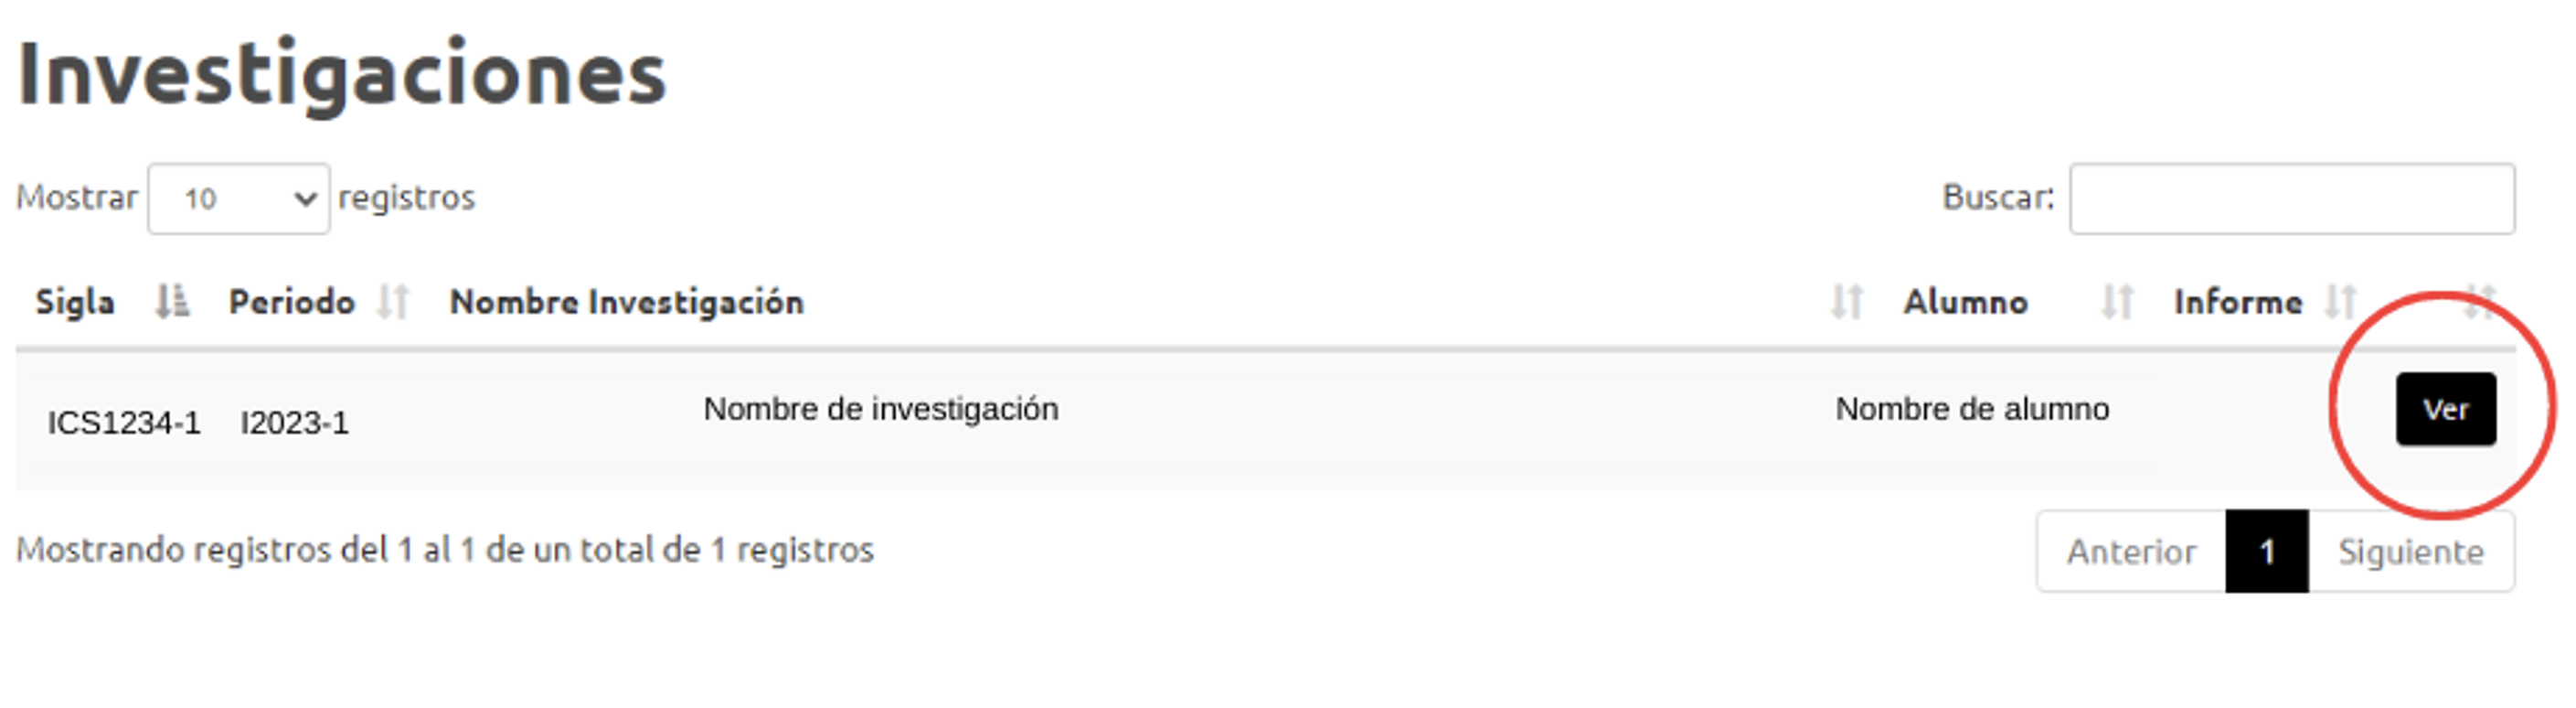
\includegraphics[width=6.13687in,height=1.85393in]{img/Imagen_1.png}

\begin{quote}
Se abrirá el detalle de la investigación, al final encontrarás el botón ``Subir Informe de Cierre'', tienes que hacer click en él para abrir el detalle del informe de cierre, en donde podrás subir el informe y la Autorización Firmada por el mentor.
\end{quote}


\begin{itemize}
  \item \underline{\textbf{Plazo de entrega}}: Dado que puedes inscribir tu Ipre durante cualquier momento del año en la plataforma Gestión Ipre, la limitante en la entrega del informe dependerá del momento en que hayas creado la investigación, obtengas un NRC e inscribas la Ipre en la plataforma Banner UC.
   Es decir, si inscribiste la IPre en Banner UC durante el periodo de inscripción de cursos para el segundo semestre, tu fecha límite de entrega del informe será al final del periodo académico del segundo semestre.\\
    Si inscribiste la IPre en Banner UC durante el periodo de inscripción de cursos para el primer semestre del siguiente año, tu fecha límite de entrega del informe será al final del periodo académico del primer semestre del siguiente año.\\
    \textbf{El no cumplimiento en la entrega del informe puede impedir la inscripción de cursos IPre en el futuro}


  \item\underline{\textbf{Extensión}}: el informe no debe contener más allá de 2.000 palabras, incluyendo resumen y cuerpo principal del artículo. Leyendas de figuras, bibliografía, autores, afiliaciones y la tabla de información incluida en este archivo no se consideran en la extensión indicada. \textbf{Informes que no respeten la extensión máxima no serán considerados}.
  \item\underline{\textbf{Figuras y tablas}}: puede incluir un máximo de 3 figuras y/o tablas para comunicar sus resultados. Las figuras y tablas deben incluir una leyenda apropiada para guiar al lector en la comprensión de sus resultados.
  \item\underline{\textbf{Estructura del escrito}}: Este informe está preparado con instrucciones para guiarlo en el uso de sus secciones de acuerdo a criterios estándar para una publicación científica. No altere la estructura indicada. Utilice las secciones y sub-secciones suministradas para facilitar la comprensión de sus resultados. \textbf{Procure usar adecuadamente el lenguaje técnico y respetar las reglas de ortografía.}
  \item\underline{\textbf{Guías para el usuario}}: este documento incluye un instructivo para el uso apropiado de referencias, preparación de material gráfico y ecuaciones. Asegúrese de seguir las instrucciones aquí entregadas. \textbf{Elimine las secciones de ayuda previo al envío del documento}.
\end{itemize}

En caso de dudas respecto de este informe, puede contactar al Coordinador del Programa de Investigación en pregrado al correo ipre@ing.puc.cl.

\newpage
